\documentclass{article}
\usepackage[utf8]{luainputenc}
\usepackage[T1]{fontenc}
\usepackage[a4paper,margin=0.75in, bottom=1in]{geometry}
\usepackage{listings}
\usepackage{courier}
\usepackage{amsmath}
\usepackage{amssymb}
\usepackage{enumerate}
\usepackage{graphicx}
\usepackage{hyperref}

\begin{document}
	
	\hrulefill
	\begin{center}
		\bfseries % Fettdruck einschalten
		\sffamily % Serifenlose Schrift
		\begin{huge}
			GTI: Grundlagen der Theoretischen Informatik
		\end{huge}\\
		\begin{Large}
			Sommersemester 2017, 5. Übungsblatt
		\end{Large}\\
		\begin{small}
			Valentin Wolf, Luis Herrmann; Tutor: Kristin Knorr; Mo 12:00-14:00
		\end{small}
		
		\vspace{-10pt}
	\end{center}
	\hrulefill
	
\section*{Aufgabe 1 - \textit{Turing–Maschinen}}
\begin{enumerate}[a)]
	\item Gesucht ist eine Turing-Maschine $M$, die die Sprache $L = \{1^{3^n} | n \ge 0\}$ über $\Sigma = \{1\}$ entscheidet. Das heißt, die TM entscheidet, ob eine übergebene Unärzahl eine Kodierung einer 3er-Potenz ist. Dazu konstruieren wir folgende Turing-Maschine $M = (Q, \Sigma, \Gamma, \delta, q_0,$ \textvisiblespace $, F)$:
	
	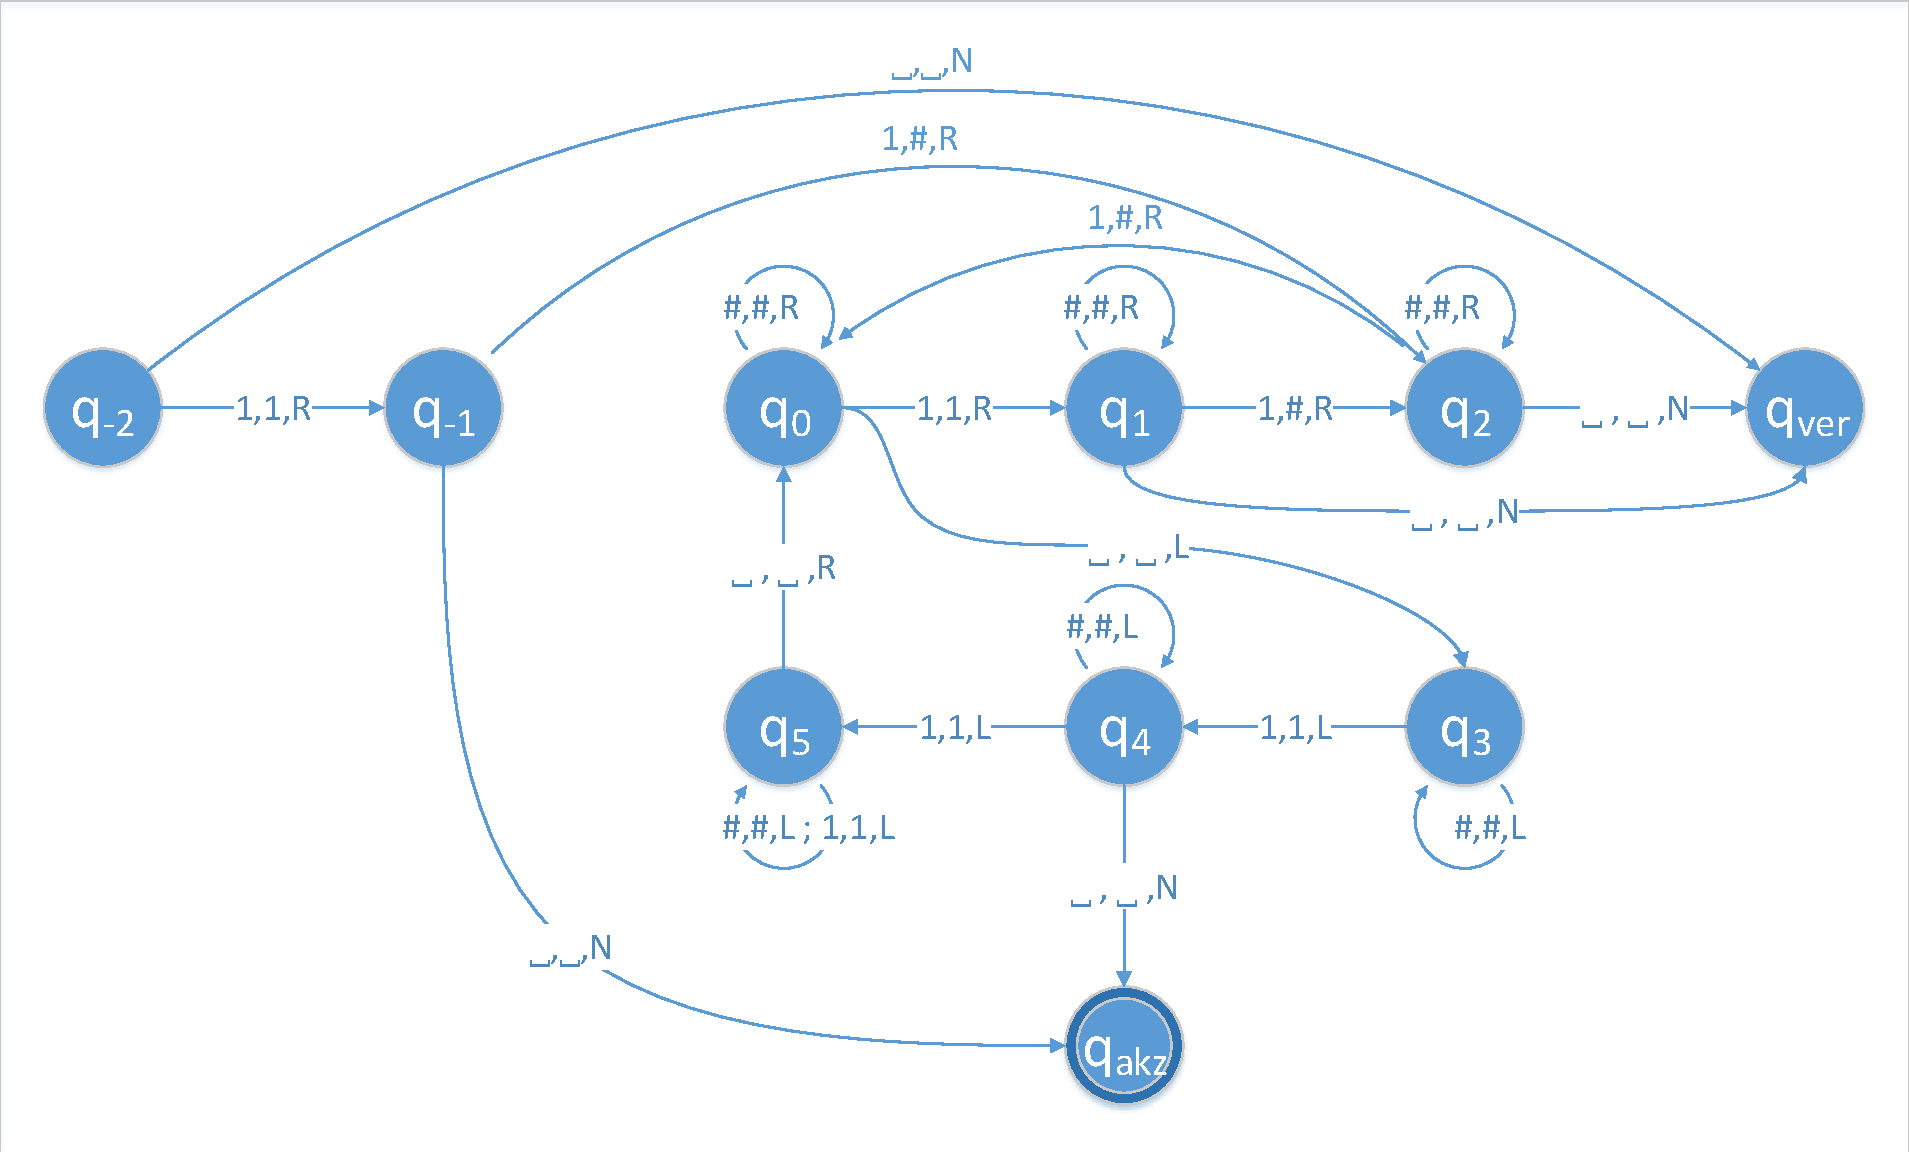
\includegraphics[width=\textwidth,page=1,trim={2 2 2 4},clip]{diagramme.pdf}
	
	Mit $\Gamma = \{1,$\textvisiblespace$, \#\}$ und $F = \{q_\text{akz}\}$. Die Idee dazu ist Folgende: Zustände $q_0$, $q_1$ und $q_2$ erfülle im Zusammenspiel mit der Zustandsüberführungsfunktion $\delta$ die Rolle eines 3-Teilers. Nehmen wir an, auf dem Band befindet sich eine Unärzahl, bei der einzelne "1" potenziell durch das Kontrollzeichen '\#' voneinander getrennt sind. Dann wird von links nach rechts jede dritte '1' (einschließlich der 0.ten) beibehalten und die 2.te und 3.te von 3 einsen in '\#' umgewandelt. Dies wird so lange wiederholt, bis ein Blank auf dem Band auftaucht. Ist dies der Fall, während wir uns in $q_1$ oder $q_2$ befinden, dann kann die Unärzahl auf dem Band nicht durch 3 teilbar sein und wir können sofort in den nicht-akzeptierenden Endzustand $q_\text{ver}$ übergehen.
	
	Falls wir uns in $q_0$ befinden, überprüfen wir mithilfe der Zustände $q_3$ bis $q_6$, ob bis zum Blank nur noch eine '1' vorhanden ist. Falls ja, heißt das, dass wir $n$-mal durch 3 teilen konnten und die 3er-Potenz $3^n$ als Eingabe erhielten; die TM geht dann in den akzeptierenden Endzustand $q_\text{akz}$ über. Folgen noch weitere '1', so ist eine Zahl größer als 1 übrig geblieben und es gilt erneut zu überprüfen, ob diese durch 3 teilbar ist. Wir bewegen uns mittels $q_5$ an das andere Ende des Bandes und beginnen in $q_0$ die Division durch 3 von Neuem.
	
	\item Wir simulieren eine beidseitig unendliche Turing-Maschine $M = (Q, \Sigma, \Gamma, \delta, q_0, \text{\textvisiblespace}, F)$ durch eine einseitig unendliche Zweispur-Turingmaschine. Wir nehmen dabei an, dass das Band nach links beschränkt ist und das linke Ende des Bandes durch das Steuerzeichen $(\#,\#)$ markiert wird. Dabei kann sich die TM in zwei Modi befinden: Im ersten Modus rechnet sie auf der "obigen" Spur und ignoriert Zeichen auf der "unteren" Spur. Kommt die TM im ersten Modus an das linke Ende und liest das Steuerzeichen $(\#,\#)$, so geht sie eine Position nach rechts und wechselt in den zweiten Modus. Im zweiten Modus werden dabei gespiegelt zum ersten Modus auf der "unteren" Spur gerechnet und Zeichen auf der "obigen" Spur ignoriert, wobei die Richtungen für Bewegungen vertauscht werden. Bewegt man sich nun nach "R", bzw. "L" und liest das Steuerzeichen $(\#,\#)$, so bewegt man sich eine Position nach rechts und rechnet im ersten Modus weiter.
	
	\item Sei $A = (Q, \Sigma, q_0, \delta, F)$ ein dfa. Dann definieren wir die TM $\tilde{A} := (\tilde{Q}, \Sigma, \Gamma, \tilde{\delta}, q_0, \text{\textvisiblespace}, \tilde{F})$ mit $\tilde{Q} = Q \cup \{q_\text{akz},q_\text{ver}\}$, $\Gamma = \Sigma \cup \{\text{\textvisiblespace}\}$ und $\tilde{F} = \{q_\text{akz}\}$ und ferner:
	
	\begin{align}
		\tilde{\delta}(q,a) = \begin{cases}
			(\delta(q,a),a,R), & a\in \Sigma\\
			(q_\text{ver},\text{\textvisiblespace},N), &q \not\in F \land a = \text{\textvisiblespace}\\
			(q_\text{akz},\text{\textvisiblespace},N), &q \in F \land a = \text{\textvisiblespace}\\
		\end{cases}
	\end{align}
	
	Sobald das erste Blank gelesen wird ist das Ende des Bands erreicht und die Berechnung endet auf dem nicht-akzeptierenden Endzustand $q_\text{ver}$ falls der aktuelle Zustand ein nicht-akzeptierender Zustand in $A$ ist und sonst im akzeptierenden Zustand $q_\text{akz}$. Da für $q_\text{ver}$ und $q_\text{akz}$ keine Nachfolgezustände in der Übergangsfunktion $\tilde{\delta}$ definiert sind, hält die Berechnung in diesen Zuständen auch tatsächlich an.
	
	\item Wir nehmen an, dass die Zahl in unärer Kodierung übergeben wird. Falls die Kodierung die Länge 1 hat, wird sie verworfen. Sonst kopieren wir die Zahl links von der Eingabe, getrennt durch einen Separator $*$. Die ersten 2 Stellen links vom Separator werden durch '0' markiert und kodieren unär die 2. Z.B.: '... \textvisiblespace11111 \textvisiblespace...' $\to$ '... \textvisiblespace11100 * 11111 \textvisiblespace...'.
	
	Dann markieren wir z.B. mit '\#' jede 2te Stelle in der rechten Zahl. Falls wir '\textvisiblespace' erreichen und das Zeichen in der vorhergehenden Zelle markiert wurde, dann wissen wir, dass die übergebene Zahl durch 2 teilbar ist und somit keine Primzahl.
	
	Sonst gehen wir links von "*" und erhöhen die Anzahl der '0' um 1 und erhalten eine natürliche Zahl $n+1$. Wir testen für diese wieder Teilbarkeit. Falls wir beim Erhöhen der 0 links auf '\textvisiblespace' stoßen, haben wir für alle Zahlen von $2 bis x$, wobei $x$ die übergebene Zahl ist, ohne Erfolg auf Teilbarkeit getestet und sind fertig. Wir löschen alle Zeichen, schreiben 1 aufs Band, gehen in akzeptierenden Endzustand und sind fertig.
	
	Offenbar handelt es sich um eine etwas ineffiziente Realisierung des Sieb des Erathostenes. Da wir nicht bis $\sqrt{n}$ prüfen können, prüfen wir stattdessen bis $n$. Die Laufzeit beträgt in der Realisierung als TM dann etwa $\mathcal{O}(n^2)$. (Im Schlimmsten Fall $n$-mal $n$ Stellen markieren.)
\end{enumerate}


\section*{Aufgabe 2 - \textit{Eine sonderbare, aber Turing–berechenbare Funktion}}

Der Einfachheit halber konstruieren wir die TM als TM mit abzählbar unendlich vielen Bändern und zugehörigen Köpfen $K$ und gehen davon aus, dass die $\Pi$ in Dezimalstellenkodierung übergeben wird, wobei sich auf Band $B_i$ die Stellen $ i, i+1, ... i+n$ befinden. Wir brauchen im Wesentlichen nur 3 Zustände $q_0, q_\text{akz}, q_\text{ver}$, von denen nur $q_\text{akz}$ akzeptierender Zustand ist. Unsere Zustandsüberführungfunktion macht nun folgendes:

\begin{enumerate}[1.]
	\item Falls kein $i$ existiert, sodass $K_i$ eine 5 liest, bewege $K_0$ nach rechts bis es '\textvisiblespace' liest und beende im nicht-akzeptierenden Zustand $q_\text{ver}$.
	
	\item Falls ein $i$ existiert sodass $K_i$ eine 5 liest, für alle Köpfe, die 5 gelesen haben: Schreibe '5', bewege den Kopf nach rechts. Für alle Köpfe, die $a \neq 5$ gelesen haben: Schreibe '$a$', bewege Kopf nach rechts. Ende im Zustand $q_0$.
	
	\item Falls alle Köpfe '\textvisiblespace' lesen und aktueller Zustand $q_0$, bewege Kopf nach rechts und gehe über in akzeptierenden Endzustand $q_\text{akz}$.
\end{enumerate}


\end{document}